%inizio capitolo 2
\chapter{Algoritmo di gestione dinamica applicato ad un singolo incrocio}

In questo capitolo si vuole analizzare il comportamento dello stesso incrocio visto in precedenza con un algoritmo di gestione ottimizzata, che conti il numero di auto in ciascuna corsia e in base a questo e ad altri parametri conceda il verde per un numero di secondi variabile. È da precisare che l’algoritmo utilizzato si basa su quello proposto da \textit{Maram Bani Younes e Azzedine Boukerche}\cite{itlc}, tuttavia sono state effettuate alcune importanti modifiche, che verranno analizzate nel corso della trattazione. 

Si è previsto,  oltre che un raffronto fra l'algoritmo di gestione statica e quello sviluppato in autonomia, modificando quanto proposto dai due ingegneri, anche un meccanismo per valutare l'efficacia di queste modifiche, confrontando il nuovo codice con una implementazione di quello presente nella pubblicazione citata. Tutti i confronti, con i relativi grafici e le relative conclusioni, verranno presentati alla fine di questo capitolo, dopo aver descritto nel dettaglio tutti gli aspetti relativi alle modifiche apportate al modello e ai meccanismi implementativi adottati.


Per quanto riguarda lo pseudocodice progettato dai due ingegneri, è disponivile alla seguente pagina.
\newpage
\begin{lstlisting}[language=C,label=pseudocode,caption=Pseudocodice di gestione dinamica di un incrocio]
while d_i di una qualsiasi corsia > 0 do
{
	
	sia j la corsia con il maggior numero di macchine;
	siano i_1 e i_2 le due corsie complementari;
		if (d_i_1 > d_i_2)
		{
			schedula j,i_1;
			d_i_1 = 0;
			t_i_1 = 0;
		}
		
		else
		{
			schedula j,i_2;
			d_i_2 = 0;
			t_i_2 = 0;
		}
		d_j = 0;
		t_j = 0;
	
}   
\end{lstlisting}
\newpage
\section{Breve spiegazione dell'algoritmo originale}
La proposta di \textit{Maram Bani Younes e Azzedine Boukerche} si basa sulla definizione di alcuni parametri, il primo dei quali è la così detta \textit{Ready Area}. Tale area è sostanzialmente il range entro il quale le macchine si possono considerare in coda per l’incrocio: si individua, per ogni semaforo della giunzione, una distanza massima, di solito corrispondente alla portata del dispositivo di rilevazione in termini di veicoli, oltre la quale le vetture non vengono più conteggiate. 

Il dispositivo in questione può essere rappresentato da una semplice telecamera che, mediante meccanismi tipici della Computer Vision, utilizzando API quali Google Vision\cite{google_vision} o OpenCV\cite{open_CV}, riesca ad individuare la variabile principale su cui si basa l’algoritmo: il numero di auto in coda per ciascuna corsia. L’implementazione hardware di questo sistema, tuttavia, non è oggetto di questa tesi e dunque non ci si dilungherà oltre nella sua spiegazione.

Il tempo concesso alle corsie prescelte (durata della luce verde) è poi dinamico, e viene calcolato sulla base della seguente formula: 

\begin{equation} \label{eq:}
  T = \theta + \frac{F_d}{S_{tf}}
\end{equation}

Il parametro $\theta$ è una costante, e rappresenta il tempo che mediamente è necessario alla prima macchina per partire, mentre $F_d$ è la distanza del veicolo più lontano dal semaforo (sempre interno alla \textit{Ready Area} ). In ultimo, $S_{tf}$ è la velocità media del flusso di auto nell’intersezione. Come è ovvio notare, sia $\theta$ che $S_{tf}$ sono ottenuti mediante delle stime, non essendo misurabili prima della effettiva esecuzione dell’algoritmo. 

Una proposta alternativa, certamente più efficiente ma anche meno facile da implementare, è quella di permettere alle automobili di comunicare fra loro e con il semaforo dati quali la $F_d$ (distanza), nonché la loro velocità media. Certamente in questo modo si renderebbe l’esecuzione dello script più veritiera ed affidabile, ed in futuro, grazie agli sforzi delle case automobilistiche, probabilmente tutto ciò sarà possibile.

Altri parametri da considerare sono $d_i$ che rappresenta il numero di automobili in coda nella corsia i-esima e $t_i$, tempo richiesto a tutti i veicoli della corsia i-esima (all’interno della \textit{Ready Area}) per lasciare l’intersezione.

\textbf{Il funzionamento dell’algoritmo è dunque il seguente:} si individua la corsia più affollata fra quella che presentano almeno un’automobile, e contestualmente si rintracciano le due corsie compatibili con essa, così come spiegato nel \textit{Capitolo \ref{capitolo1}} e come si può notare nella \textit{figura \ref{dirCompatibili}}.

A questo punto, fra queste due candidate si sceglie ancora la più affollata; in questo modo non solo si va a concedere il verde alla strada con più automobili, ma si cerca anche di ottimizzare la scelta della sua complementare, che non resta statica (come invece è nell’algoritmo utilizzato nel capitolo precedente), ma diventa dinamica ed intelligente. Successivamente l’algoritmo prevede di calcolare il tempo \textit{T}, concedendolo alla luce verde delle due corsie, e di azzerare le variabili $d_i, d_j$ e $t_i, t_j$ relative, in quanto si prevede che dopo T secondi le corsie in questione presentino un numero di veicoli pari a zero.
\newpage
\section{Le modifiche apportate}
Sono molteplici le modifiche apportate all’algoritmo proposto, alcune delle quali a puro scopo implementativo, altre come migliorie.

In primo luogo, si è preferito non considerare una \textit{Ready Area} per non dover dare alle code di \textit{Simulink} un massimo numero di entità (veicoli) da contenere, questo per effettuare più simulazioni variando i tassi di generazione, verificando il comportamento del modello anche in condizioni esageratamente negative, con code anche molto affollate (più di 50 automobili). 

Il concetto della \textit{Ready Area}, tuttavia, non è stato abbandonato del tutto, ma è stato piuttosto migliorato: si è deciso di concedere un tempo minimo ed un tempo massimo alla durata del verde per ciascuna corsia. Il tempo minimo serve perché, anche con una sola macchina in coda, si è voluto stabilizzare la situazione, che altrimenti si sarebbe tradotta in un passaggio troppo repentino dal verde al rosso. Per quanto concerne il tempo massimo, questo è diretta espressione della \textit{Ready Area}: invece che considerare un massimo numero di veicoli, si considera che, indipendentemente da questo numero, il verde non può durare più di un certo valore, questo per evitare tempi di attesa troppo lunghi nelle corsie meno affollate, ma comunque in cui sono presenti veicoli. 

Il tempo concesso alla luce verde, poi, viene calcolato tenendo conto della distribuzione uniforme che governa gli \textit{Entity Server}, precedentemente descritta, assegnando ad ogni macchina un valore pari al valore medio della distribuzione (in questa simulazione pari a $5s$), ed ottenendo il tempo complessivo moltiplicando questo valore per il numero di veicoli in coda. A questo punto, se il numero ottenuto è inferiore al tempo minimo, esso si scarta, e si prende in considerazione proprio quel minimo, viceversa se supera il tempo massimo è questo ad essere tenuto in considerazione e ad essere concesso. Pertanto, poiché non è detto che le code a cui viene dato il via libera si svuotino, non si va ad azzerare i contatori relativi, ma semplicemente all'esecuzione successiva della funzione questi sono aggiornati con i nuovi dati rilevati, ottenuti dalle code stesse.

Inoltre, è stata individuata una grande lacuna nell’algoritmo oggetto della pubblicazione citata: l’assenza di un meccanismo di gestione della \textit{starvation}. 

Considerando esclusivamente il \textit{codice \ref{pseudocode}}, infatti, si nota che se in una strada continuano a confluire veicoli più velocemente che nelle altre, a questa sarà sempre concesso il verde. Questo comportamento da un lato è positivo perché si va a decongestionare tale corsia, ma è ovviamente improponibile, in quanto potrebbe paradossalmente capitare che un semaforo resti rosso per ore ed ore, e che una persona sia costretta ad attendere un tempo esagerato prima di passare, perché la sua strada è meno affollata.

È stato scelto dunque di implementare un meccanismo di gestione della \textit{starvation} mediante un algoritmo \textit{LRU} (Least Recently Used) opportunamente modificato. Ad ogni corsia è associato un contatore, ed ogni qual volta ad una strada viene concesso il verde, il suo contatore viene azzerato, mentre quello delle altre si incrementa del numero di secondi per cui è stato concesso il verde alla corsia suddetta. In questo modo, quando un contatore raggiunge un valore limite (liberamente impostabile), la relativa strada ottiene priorità massima, e l’algoritmo viene applicato in maniera identica (calcolo del tempo del verde e selezione della complementare) come se essa fosse quella più affollata.

È anche da notare che sono stati apportati alcuni minimi cambiamenti al modello: le code sono state collegate agli ingressi del blocco contenente la funzione da eseguire, comunicando ad essa il numero di veicoli presenti, ed il canale di \textit{feedback} è stato utilizzato per implementare il meccanismo della gestione della \textit{starvation}, e non per conoscere a quale semaforo è stato concesso il verde nell’esecuzione precedente, informazione ora inutile. Non è stato variato altro, se non, ovviamente, il codice nel blocco \textit{Matlab Function}, quindi non si ravvisa la necessità di approfondire nuovamente la necessità di descrivere nei dettagli nuovamente l'intero modello, il cui schema è comunque presente alla pagina seguente, seguito dal codice che lo governa.

\begin{figure}[H]
  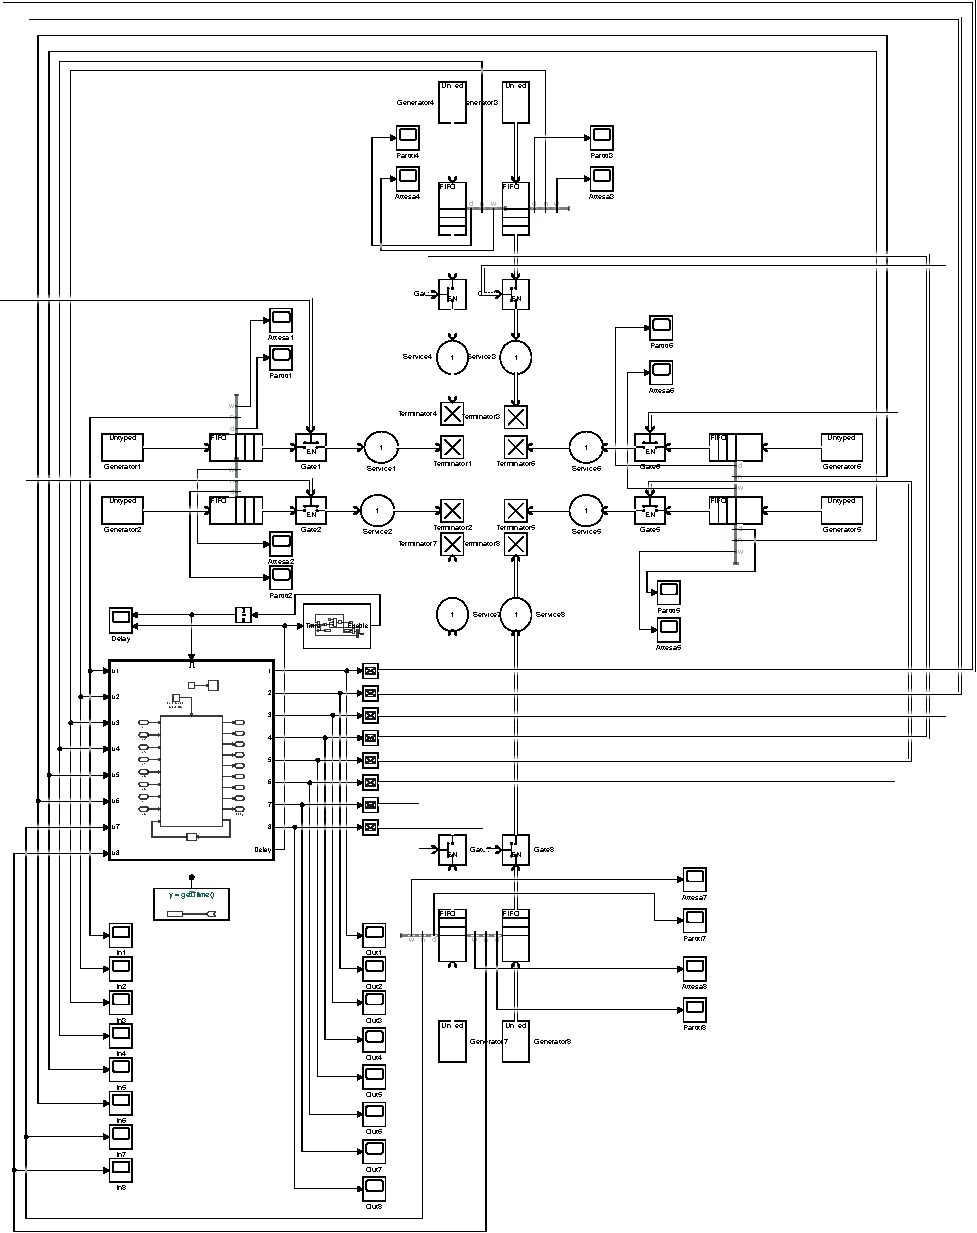
\includegraphics[width=1\textwidth]{SingoloIncrocioAlgoritmo.pdf}
  \caption{Modello di un incrocio a raso a quattro bracci in Simulink e SimEvents, gestione dinamica}
  \label{fig:modellosingoloincrocioalgoritmo}
\end{figure}
\newpage

\begin{lstlisting}[language=Matlab,label=key,caption=Implementazione dell'algoritmo di gestione dinamica di un singolo incrocio]
function [delay, y1, y2, y3, y4, y5, y6, y7, y8, feedback] = fcn(u1, u2, u3, u4, u5, u6, u7, u8, history)


% VARIABILI DI USCITA
% Prima attesa, prima dell'esecuzione dell'algoritmo la prima volta
delay = 1; 
y1 = 0; 
y2 = 0; 
y3 = 0; 
y4 = 0; 
y5 = 0; 
y6 = 0; 
y7 = 0;
y8 = 0;
feedback = zeros([4 2]);
 
% Numero di veicoli per ogni direzione
M = ([u1 u2; u3 u4; u5 u6; u7 u8;]);
 
% Tempo medio per fluire per ogni macchina
Tv = 5;
 
% Massimo tempo del verde
MaxGreen = 60;
 
% Minimo tempo del verde
MinGreen = 10;
 
% Controllo sulla starvation (LRU). Tempo di attesa massimo: 5 minuti
starvation = 300;
 
% Cerco il massimo
[R, C] = size(M);
iMax = 1;
jMax = 1;
vMax = M(1, 1);
 
%Usato per la starvation, interrompe la ricerca
flag = 0;
 
for i = 1 : 1 : R
    for j = 1 : 1 : C
        
        if M(i, j) > 0 && history(i, j) > starvation
            vMax = M(i, j);
            iMax = i;
            jMax = j;
            flag = 1;
            break;
        end
 
        if M(i, j) > vMax
            vMax = M(i, j);
            iMax = i;
            jMax = j;
        end
       
    end
    
    if flag == 1
        break;
    end
end
 
 
% Cerco i possibili candidati
[c1_i, c1_j, c2_i, c2_j] = getCandidates(iMax, jMax);
 
%Scelgo tra i candidati
if M(c1_i, c1_j) > M(c2_i, c2_j) 
    iCan = c1_i;
    jCan = c1_j;
else
    iCan = c2_i;
    jCan = c2_j;
end
 
delay = vMax*Tv;
 
if vMax*Tv > MaxGreen
        delay = MaxGreen;
elseif vMax*Tv < MinGreen
        delay = MinGreen;
end
    
%Risultato
U = ([0 0; 0 0; 0 0; 0 0]);
 
U(iMax, jMax) = 1;
U(iCan, jCan) = 1;
     
history( : ) = history( : ) + delay;
    
history(iMax, jMax) = 0;
history(iCan, jCan) = 0;

%Output 
y1 = U(1, 1); y2 = U(1, 2); y3 = U(2, 1); y4 = U(2, 2); y5 = U(3, 1); y6 = U(3, 2); y7 = U(4, 1); y8 = U(4, 2); feedback(:) = history(:);
end
    
\end{lstlisting}
\newpage
\section{Spiegazione del codice implementato}
In primo luogo vengono inizializzate le variabili in uscita della funzione, corrispondenti al valore di trigger degli otto entity gate rappresentanti le varie corsie. Di default questi valori sono posti a 0 (semaforo rosso). In input si accetta il numero di veicoli presenti in ogni coda nell'istante in cui la funzione viene richiamata, nonché il vettore \textit{history}, usato per gestire la starvation, il cui significato sarà chiaro più avanti.

I due \textit{cicli for} annidati servono ad individuare la strada con il numero di veicoli più elevato, purché non si verifichi il caso di \textit{starvation}. Tale strada (individuata da due indici, \textit{i} e \textit{j} all’interno della matrice \textit{M}, matrice che organizza gli otto input indipendenti), viene poi data in pasto alla funzione \textit{getCandidates}, il cui codice è alla pagina seguente e che restituisce gli indici relativi alla matrice M che individuano le due strade che possono essere scelte assieme alla principale. A questo punto fra le due corsie complementari candidate viene scelta, come già detto, quella più affollata. Viene calcolato il tempo da concedere al verde in funzione del numero di veicoli della strada scelta come principale, e vengono effettuati i controlli con il tempo minimo ed il tempo massimo, precedentemente dichiarati come costanti.

Successivamente, ogni elemento del vettore \textit{History}, il quale contiene i contatori inerenti all’algoritmo \textit{LRU} per ogni corsia, viene incrementato del tempo stabilito, azzerando poi gli elementi corrispondenti alle corsie a cui si sta concedendo il verde.

In output viene inviato \textit{1} agli \textit{Entity Gate} che devono aprirsi, corrispondenti alle strade individuate, e \textit{0} a tutti gli altri. 

Oltre a queste informazioni rappresenta un output anche il \textit{delay}, ovvero proprio il tempo concesso, che viene inviato al timer descritto nel \textit{capitolo \ref{capitolo1}}, che richiamerà la funzione allo scadere dello stesso.
\newpage
\begin{lstlisting}[language=Matlab,label=key,caption=Scelta delle due strade complementari a quella selezionata come principale]
    function [i1, j1, i2, j2] = getCandidates(i, j)
    % Direzioni accoppiate (8x4)
    % Per ciascuna direzione scelta, ci sono 2 possibili direzioni
    % complementari
    % D = {[1 2; 3 1] [1 1; 3 2]; [4 1; 2 2] [2 1; 4 2]; [3 2; 1 1] [3 1; 1 2]; [4 2; 2 1] [4 1; 2 2]};
    
    i1 = 0;
    i2 = 0;
    j1 = 0;
    j2 = 0;
    
    if i==1 && j ==1
        i1 = 1;
        j1 = 2;
        i2 = 3;
        j2 = 1;
    elseif i==1 && j==2
       i1 = 1;
       j1 = 1;
       i2 = 3;
       j2 = 2;
    elseif i==2 && j==1
       i1 = 4;
       j1 = 1;
       i2 = 2;
       j2 = 2;
    elseif i==2 && j==2
       i1 = 2;
       j1 = 1;
       i2 = 4;
       j2 = 2;
    elseif i==3 && j==1
       i1 = 3;
       j1 = 2;
       i2 = 1;
       j2 = 1;
    elseif i==3 && j==2
       i1 = 3;
       j1 = 1;
       i2 = 1;
       j2 = 2;
    elseif i==4 && j==1
       i1 = 4;
       j1 = 2;
       i2 = 2;
       j2 = 1;
    elseif i==4 && j==2
       i1 = 4;
       j1 = 1;
       i2 = 2;
       j2 = 2;
    end
            
        
end
\end{lstlisting}

È da sottolineare che questo codice funziona fintanto che gli ingressi non vengono variati: se si dovesse collegare una strada ad un ingresso diverso da quello previsto ed utilizzato nella simulazione chiaramente l’intero algoritmo non sarebbe più affidabile. L'autore di questa tesi è consapevole che esistono metodi più eleganti ed ottimizzati rispetto a questa sequenza di \textit{if} ed \textit{elseif} per ottenere il medesimo scopo, tuttavia si è reso necessario procedere in questo modo per lo scarso supporto del linguaggio \textit{Matlab} a tali meccanismi, come, per esempio, gli \textit{switch - case}. In questo modo, inoltre, il codice risulta particolarmente leggibile e facile da comprendere.
\newline

Le differenze con un normale algoritmo di gestione di una giunzione, come quello proposto nel \textit{capitolo \ref{capitolo1}} sono quindi evidenti: in primo luogo non si segue una turnazione statica per quanto riguarda la concessione del verde, seguendo invece un meccanismo di priorità: ci si chiede infatti quale sia la strada che necessita del verde in quell'istante, più delle altre, e glielo si concede. Inoltre anche il tempo per cui questo verde è concesso è variabile: si ipotizzi per esempio di analizzare l'incrocio durante le ore notturne, non avrebbe senso concedere il verde per un numero di secondi elevato quando in coda è presente una sola macchina, si tratterebbe di una perdita di tempo, tradotta in un maggior consumo di carburante ed un maggiore stress per gli automobilisti delle altre corsie, costretti ad attendere perché viene concesso il verde ad una strada praticamente vuota. Viceversa è ovvio che durante il giorno, per una strada affollata, la durata della luce verde deve essere sufficiente da garantire che un buon numero delle macchine in coda defluisca.
\newpage

\section{Il modello per confrontare le diverse gestioni del singolo incrocio}

I benefici esposti, ovviamente, devono trovare riscontro in un confronto imparziale ed assolutamente valido fra i modelli presentati, affinché a partire dai medesimi dati in input (le automobili generate), e con gli stessi parametri (tasso di generazione, tempo di servizio interno agli \textit{Entity Server}) essi gestiscano l'incrocio secondo la propria logica. Si è scelto, pertanto, di creare in un nuovo workspace il modello identificato dalla figura a pagina seguente \textbf{INSERIRE NUMERO}. Si può notare come al suo interno siano presenti tre blocchi principali, ognuno dei quali è rappresentativo di un algoritmo di gestione. Cliccando infatti nei tre blocchi presenti, di tipo \textit{Subsystem}, si comprende subito come questi siano in realtà esattamente i modelli precedentemente descritti. Il primo, quello più in alto, è quello presentato nel \textit{capitolo \ref{capitolo1}}, relativo ad una gestione statica (\textit{figura \ref{fig: modelloSingoloIncrocio}}). Quello in basso a sinistra invece si riferisce al modello di controllo dinamico, di cui si è parlato in questo capitolo (\textit{figura \ref{fig:modellosingoloincrocioalgoritmo}}), mentre quello in basso a destra è perfettamente identico a quest'ultimo, eccezion fatta per la gestione della starvation, che si è eliminata. Ciò è stato fatto per capire come tale gestione, che comunque resta assolutamente necessaria, interferisca con il normale funzionamento dell'algoritmo stesso.

Nello specifico, in questo terzo modello, si è provveduto semplicemente a commentare la seguente porzione di codice, lasciando tutto il resto invariato.
\newline
\begin{lstlisting}[language=Matlab,label=starvation,caption= Porzione di codice relativa alla gestione della starvation]
    if M(i, j) > 0 && history(i, j) > starvation
            vMax = M(i, j);
            iMax = i;
            jMax = j;
            flag = 1;
            break;
    end
        ...
        ...
        ...
   if flag == 1
        break;
   end
\end{lstlisting}

Gli \textit{Entity Generator}, poi, sono stati spostati all'esterno, e collegati a dei blocchi di tipo \textbf{Entity Replicator\cite{entityreplicator}}, in modo tale che appena una entità viene generata in una corsia specifica, questa venga subito inviata ai tre modelli. In questo modo i tre incroci sono esattamente identici sia per quanto riguarda il numero di entità che devono gestire che per quanto concerne quando queste si presentano, tutto questo per garantire l'assoluta imparzialità delle condizioni, precedentemente citata.
\newline

Dunque il workflow è il seguente: quando una entità viene generata, questa viene inviata a tutti e tre gli incroci, in corrispondenza della stessa corsia e nello stesso istante di tempo. La simulazione parte allo stesso istante per tutti e tutti sono configurati secondo gli stessi parametri. Al termine della simulazione tutti gli incroci producono tre grafici per ogni corsia, relativi al tempo di attesa medio, al numero di macchine totali che hanno attraversato tale strada ed al numero medio di macchine in coda in funzione dell'ora del giorno. Confrontando i grafici di una stessa strada, e facendo questo per ogni strada presente, si ottiene una chiara idea di quale dei tre algoritmi stia funzionando meglio.

\newpage

\section{I risultati ottenuti}
Per le seguenti simulazioni sono stati analizzati due possibili scenari: il primo con dei tassi di generazione randomici, esattamente come presentato nel \textit{capitolo \ref{capitolo1}}, con il parametro $\mu$ scelto casualmente, secondo una distribuzione uniforme, fra 20 e 35. Questo per ottenere un numero di automobili sì variabile, ma che sia confrontabile fra le varie strade, con una configurazione dunque che può dirsi bilanciata. Il codice interno agli \textit{Entity Generator} non è dunque stato variato rispetto a quanto presentato nel \textit{codice \ref{mu-definition}}, così come la definizione dei parametri globali (\textit{codice \ref{entity-generator}}). In una configurazione di questo genere sono stati ottenuti i risultati riportati nella seguente tabella, a fronte di questi valori di $\mu$ generati.
\newline

\textbf{INSERIRE TABELLA. PER OGNI CORSIA TEMPI MEDI ATTESA E MAX MACCHINE}
\newline

Sono riportati, inoltre, alcuni grafici indicativi, relativi ad una singola corsia (sempre la stessa, quella del braccio ovest relativa alla svolta a sinistra), per ciascuno dei tre modelli, inerenti al tempo medio d'attesa ed al numero di macchine in coda in funzione dell'ora del giorno.

















